%% Based on a TeXnicCenter-Template by Gyorgy SZEIDL.
%%%%%%%%%%%%%%%%%%%%%%%%%%%%%%%%%%%%%%%%%%%%%%%%%%%%%%%%%%%%%

%------------------------------------------------------------
%
\documentclass[a4paper,12pt,leqno, notitlepage]{article}%
%Options -- Point size:  10pt (default), 11pt, 12pt
%        -- Paper size:  letterpaper (default), a4paper, a5paper, b5paper
%                        legalpaper, executivepaper
%        -- Orientation  (portrait is the default)
%                        landscape
%        -- Print size:  oneside (default), twoside
%        -- Quality      final(default), draft
%        -- Title page   notitlepage, titlepage(default)
%        -- Columns      onecolumn(default), twocolumn
%        -- Equation numbering (equation numbers on the right is the default)
%                        leqno
%        -- Displayed equations (centered is the default)
%                        fleqn (equations start at the same distance from the right side)
%        -- Open bibliography style (closed is the default)
%                        openbib
% For instance the command
%           \documentclass[a4paper,12pt,leqno]{article}
% ensures that the paper size is a4, the fonts are typeset at the size 12p
% and the equation numbers are on the left side
%
\usepackage{amsmath}%
\usepackage{amsfonts}%
\usepackage{amssymb}%
\usepackage{graphicx}
\usepackage[utf8]{inputenc}
\usepackage[magyar]{babel}
%-------------------------------------------
\frenchspacing
\sloppy

% define references
\newcommand{\figref}[1]{\ref{fig:#1}.}
\renewcommand{\eqref}[1]{(\ref{eq:#1})}
\newcommand{\listref}[1]{\ref{listing:#1}.}
\newcommand{\sectref}[1]{section \ref{sect:#1}-\nameref{sect:#1}}
\newcommand{\tabref}[1]{\ref{tab:#1}.}

\begin{document}

\title{Agilis módszertan bevezetése}
\author{Horváth András \\ Széchenyi István Egyetem, Győr}
\date{2019. november 13}
\maketitle

\begin{abstract}

Ez a dolgozat az IT projekmenedzsment tárgy teljesítéséhez készült. A dolgozatban összehasonlítom a kalsszikus és az agilis szoftver\-fejlesztési folya\-matot. Bemutatom ezek szereplőit, metódusait, alkalmazási területeit.

Ezután áttekintem a projektmenedzsment szereplőit és folyamatát. Célom bemutatni, hogy egy szoftverfejlsztéssel foglalkozó hogyan kerülhet bevezetésre az agilis módszertan. Legvégül kitérek arra kérdésre, hogy lehet-e átfedés vagy valamilyen kapcsolat a projekt-menedzseri feladatok és az agilis szoftver\-fejlesztés szerepkörei között.
\end{abstract}

\section{Szoftver\-fejlesztési módszerek}
\label{sec:s}

A dolgozat elején kettő, alapvetően különböző szoftver\-fejlesztési módszert tekintünk át. A két módszer között lényeges szemléletbeli különbségek vannak.

\subsection{Klasszikus szoftver\-fejlesztés}
\label{sec:Klasszikus}

Klasszikus szoftver\-fejlesztés alatt legtöbben a vízesés modellt értik. Ez a módszer régen nagyon elterjedt volt manapság viszont szinte elképzelhetetlen a használata összetett szoftver fejlesztése esetén. Ennek oka a módszer egyenes munkafolyamata és szigorúsága. A módszer fázisait az \figref{waterfall} ábra~\cite{waterfall_image} mutatja. Ezek az alábbiak:
\begin{description}
	\item[Szükségletek felmérése:] Ebben a fázisban a cél pontosan megérteni és dokumentálni mire van szöksége a vásárlónak.
	\item[Rendszer megtervezése:] A tervezés fázisában az előző fázisban elkészített dokumentumok alapján elő kell állítani a rendszer struktúráját.
	\item[Rendszer megvalósítása:] Ebben a fázisban történik a kódolás, a tervezett struktúra implementálása
	\item[Tesztelés:] Ebben a fázisban ellenőrizzük hogy amit implementáltunk az megegyezik a tervezettel, illetve hogy a vevő igényeit kielégíti-e.
	\item[Üzemeltetés:] Az üzemeltetés a szoftver karbantartása, utólagos fejlesztése ami a teljes ráfordítás 60\%-át is elérheti.\cite{waterfall}
\end{description}

A \cite{waterfall} forrás mindezen fázisok előtt megemlíti a megvalósíthatósági tanulmányt. Ennek célja eldönteni, hogy technológiailag lehetséges-e, illetve pénzügyileg mennyire éri meg a szoftverfejlesztésbe belefogni.

\begin{figure}[htb]
	\centering
		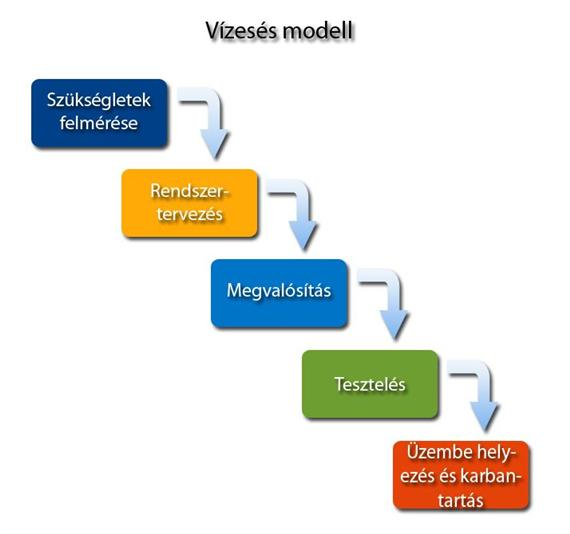
\includegraphics[width=0.85\textwidth]{images/waterfall.jpg}
	\caption{A vízesés modell fázisai \cite{waterfall_image}}
	\label{fig:waterfall}
\end{figure}

Ez a folyamat nagyon hasonlít az előadáson bemutatott álatalános projekt folyamattal. Abban szintúgy megtalálható a tervezés, megvalósítás és felügyelés lépései. A lényeges különbség az ott bemutatott folyamat és az itt leírt szofteverfejlesztési folyamat között, hogy ebben nincs lehetőség a fejlesztés megszakítására. Ez az üzleti életben nagy hátrány ebből adódik, hogy ezt a modellt nem alkalmazzák.

Ennek a modellnek egy használható változata, ha egy iteratív ciklussá alakítjuk. Az elkészített terméket a megrendelő használja, majd új követelményekkel megfogalmazza további szükségleteit. Ezután újra  a tervezés és  a megvalósítás következik. Ez lehetőséget ad a hibák kijavítására.


\subsection{Agilis szoftver\-fejlesztés}

Az 1190-as években a gyors változtatások és a felesleges munkavégzés elkerülése érdekében javasolták az agilis módszert. Az agilis szoftver\-fejlesztés valójában több fejlesztési folyamatot foglal magában. Ilyen folyamatok/módszerek például a \emph{Scrum}, \emph{eXtreme Programming} és a \emph{Lean}.\cite{agile} Ezek a módszerek valamilyen módon a fejlesztés hatékonyságának növelésére törekednek, így a projekt hamarabb és jobb minőségű szoftvert szállíthat.

A Scrum módszer lényege az iterációban és az inkrementális fejlesztésben rejlik. Nagyon hasonlóan a klasszikus vízesés modellhez, egy iterációban a 
\begin{itemize}
	\item követelmények összegyűjtése és megértése
	\item tervezés
	\item kódolás
	\item tesztelés és elfogadás
\end{itemize}
történik meg. Itt azonban mindez a változásra nyitottan történik meg. A fejlesztő csapat maga határozza meg, hogy a következő szoftver-szállítmányba adott idő alatt mit tud megvalósítani. A megrendelő a követelményet ízlése szerint priorizálhatja és a csapat az alapján fog sorban menni  a tervezés során. A szállítmányt a megrendelő kipróbálja és a következő tervezésre már vissza is tud jelezni és új követelményeket megfogalmazni.

\section{A szoftver\-fejlesztés mint projekt}

Az előzőekben bemutatott metodológiák után most tekintsünk a szoftverfejlesztésre, mint projektre. Minden projektre jellemző, hogy időben és célkitűzésében elhatárolható. Ez a kitétel egy szoftver fejlesztésére igaz lehet, de nem minden esetben. Pl.: egy operációs rendszer megalkotása rengeteg munka, és a ma leggyakrabban használtak már több évtizede fejlődnek. Egy mobil-játék lefejlesztése tipikusan sokkal hamarabb megvan, és többsége ha egyszer elkészült úgy is marad, befejezettnek van tekintve.

Jómagam a Knorr-Bremse DAS (Driver Assistance System) csoportjában dolgozom.

\bibliography{biblio}{}
\bibliographystyle{plain}

\end{document}
